\documentclass[10pt]{beamer}

% Packages
\usepackage[utf8]{inputenc}
\usepackage[T1]{fontenc}
\usepackage{amsmath, amssymb, amsthm}
\usepackage{graphicx}
\usepackage{booktabs}
\usepackage{hyperref}
\usepackage{tikz}
\usetikzlibrary{shapes,arrows,positioning}

% Theme settings
\usetheme{default}
\usecolortheme{default}
\usefonttheme{professionalfonts}

\definecolor{ImperialBlue}{RGB}{0, 62, 116}
\definecolor{DarkGray}{RGB}{51, 51, 51}
\definecolor{LightGray}{RGB}{245, 245, 245}
\definecolor{AccentOrange}{RGB}{214, 96, 77}
\definecolor{AccentGreen}{RGB}{46, 139, 87}

% Apply colors
\setbeamercolor{frametitle}{fg=ImperialBlue, bg=white}
\setbeamercolor{title}{fg=ImperialBlue}
\setbeamercolor{structure}{fg=ImperialBlue}
\setbeamercolor{normal text}{fg=DarkGray}
\setbeamercolor{block title}{fg=white, bg=ImperialBlue}
\setbeamercolor{block body}{fg=DarkGray, bg=LightGray}
\setbeamercolor{itemize item}{fg=ImperialBlue}
\setbeamercolor{enumerate item}{fg=ImperialBlue}

% Remove navigation symbols
\setbeamertemplate{navigation symbols}{}

% Customize frame title
\setbeamertemplate{frametitle}{
  \vspace{0.5em}
  \insertframetitle
  \vspace{0.3em}
}

% Customize itemize
\setbeamertemplate{itemize items}[circle]
\setlength{\leftmargini}{1.5em}

% Footer
\setbeamertemplate{footline}{
  \leavevmode%
  \hbox{%
  \begin{beamercolorbox}[wd=.333333\paperwidth,ht=2.25ex,dp=1ex,left]{author in head/foot}%
    \hspace{1em}\usebeamerfont{author in head/foot}\insertshortauthor
  \end{beamercolorbox}%
  \begin{beamercolorbox}[wd=.333333\paperwidth,ht=2.25ex,dp=1ex,center]{title in head/foot}%
    \usebeamerfont{title in head/foot}\insertshorttitle
  \end{beamercolorbox}%
  \begin{beamercolorbox}[wd=.333333\paperwidth,ht=2.25ex,dp=1ex,right]{date in head/foot}%
    \usebeamerfont{date in head/foot}\insertshortdate{}\hspace*{2em}
    \insertframenumber{} / \inserttotalframenumber\hspace*{2ex} 
  \end{beamercolorbox}}%
  \vskip0pt%
}

% Title page customization
\setbeamertemplate{title page}{
  \vbox{}
  \vfill
  \begingroup
    \centering
    {\usebeamercolor[fg]{title}\usebeamerfont{title}\inserttitle\par}
    \vskip0.5em
    {\usebeamercolor[fg]{subtitle}\usebeamerfont{subtitle}\insertsubtitle\par}
    \vskip2em
    {\usebeamercolor[fg]{author}\usebeamerfont{author}\insertauthor\par}
    \vskip0.5em
    {\usebeamercolor[fg]{institute}\usebeamerfont{institute}\insertinstitute\par}
    \vskip1em
    {\usebeamercolor[fg]{date}\usebeamerfont{date}\insertdate\par}
  \endgroup
  \vfill
}

% Commands for highlighting
\newcommand{\emphbox}[1]{\colorbox{LightGray}{\textcolor{DarkGray}{#1}}}
\newcommand{\highlight}[1]{\textcolor{AccentOrange}{\textbf{#1}}}
\newcommand{\good}[1]{\textcolor{AccentGreen}{#1}}
\newcommand{\bad}[1]{\textcolor{AccentOrange}{#1}}

%----------------------------------------------------------------------------------------
\title{Stablecoins and Central Bank Digital Currencies}
\subtitle{ECOM215: Blockchain Economics and Digital Assets}
\author{Dr Daniele Bianchi}
\institute{Queen Mary, University of London}
\date{Semester B, 2025/2026}
%----------------------------------------------------------------------------------------

\begin{document}

\AtBeginSection[]{
  \begin{frame}[plain]
    \vfill
    \begin{center}
      {\Large\color{ImperialBlue}\insertsection}
    \end{center}
    \vfill
  \end{frame}
}

\begin{frame}[plain]
  \titlepage
\end{frame}

\begin{frame}{Today's Agenda}
  \tableofcontents
\end{frame}

%----------------------------------------------------------------------------------------
\section{Why Stablecoins?}
%----------------------------------------------------------------------------------------

\begin{frame}{The Volatility Problem}
  Recall from Topic 1: Bitcoin and other cryptocurrencies are extremely volatile.
  
  \vspace{1em}
  \textbf{This creates practical problems}:
  \begin{itemize}
    \item \textbf{Payments}: If you accept BTC for a \$100 item, it might be worth \$80 tomorrow
    \item \textbf{Lending}: How do you price a loan in an asset that moves 10\% daily?
    \item \textbf{Smart contracts}: DeFi needs a stable unit of account
  \end{itemize}
  
  \vspace{1em}
  \textbf{The solution}: Create tokens that maintain a stable value, typically pegged to \$1.
  
  \begin{block}{Stablecoin}
    A cryptocurrency designed to maintain a stable value relative to a reference asset, most commonly the US dollar.
  \end{block}
\end{frame}

\begin{frame}{Stablecoins: Market Overview}
  \begin{figure}
    \centering
    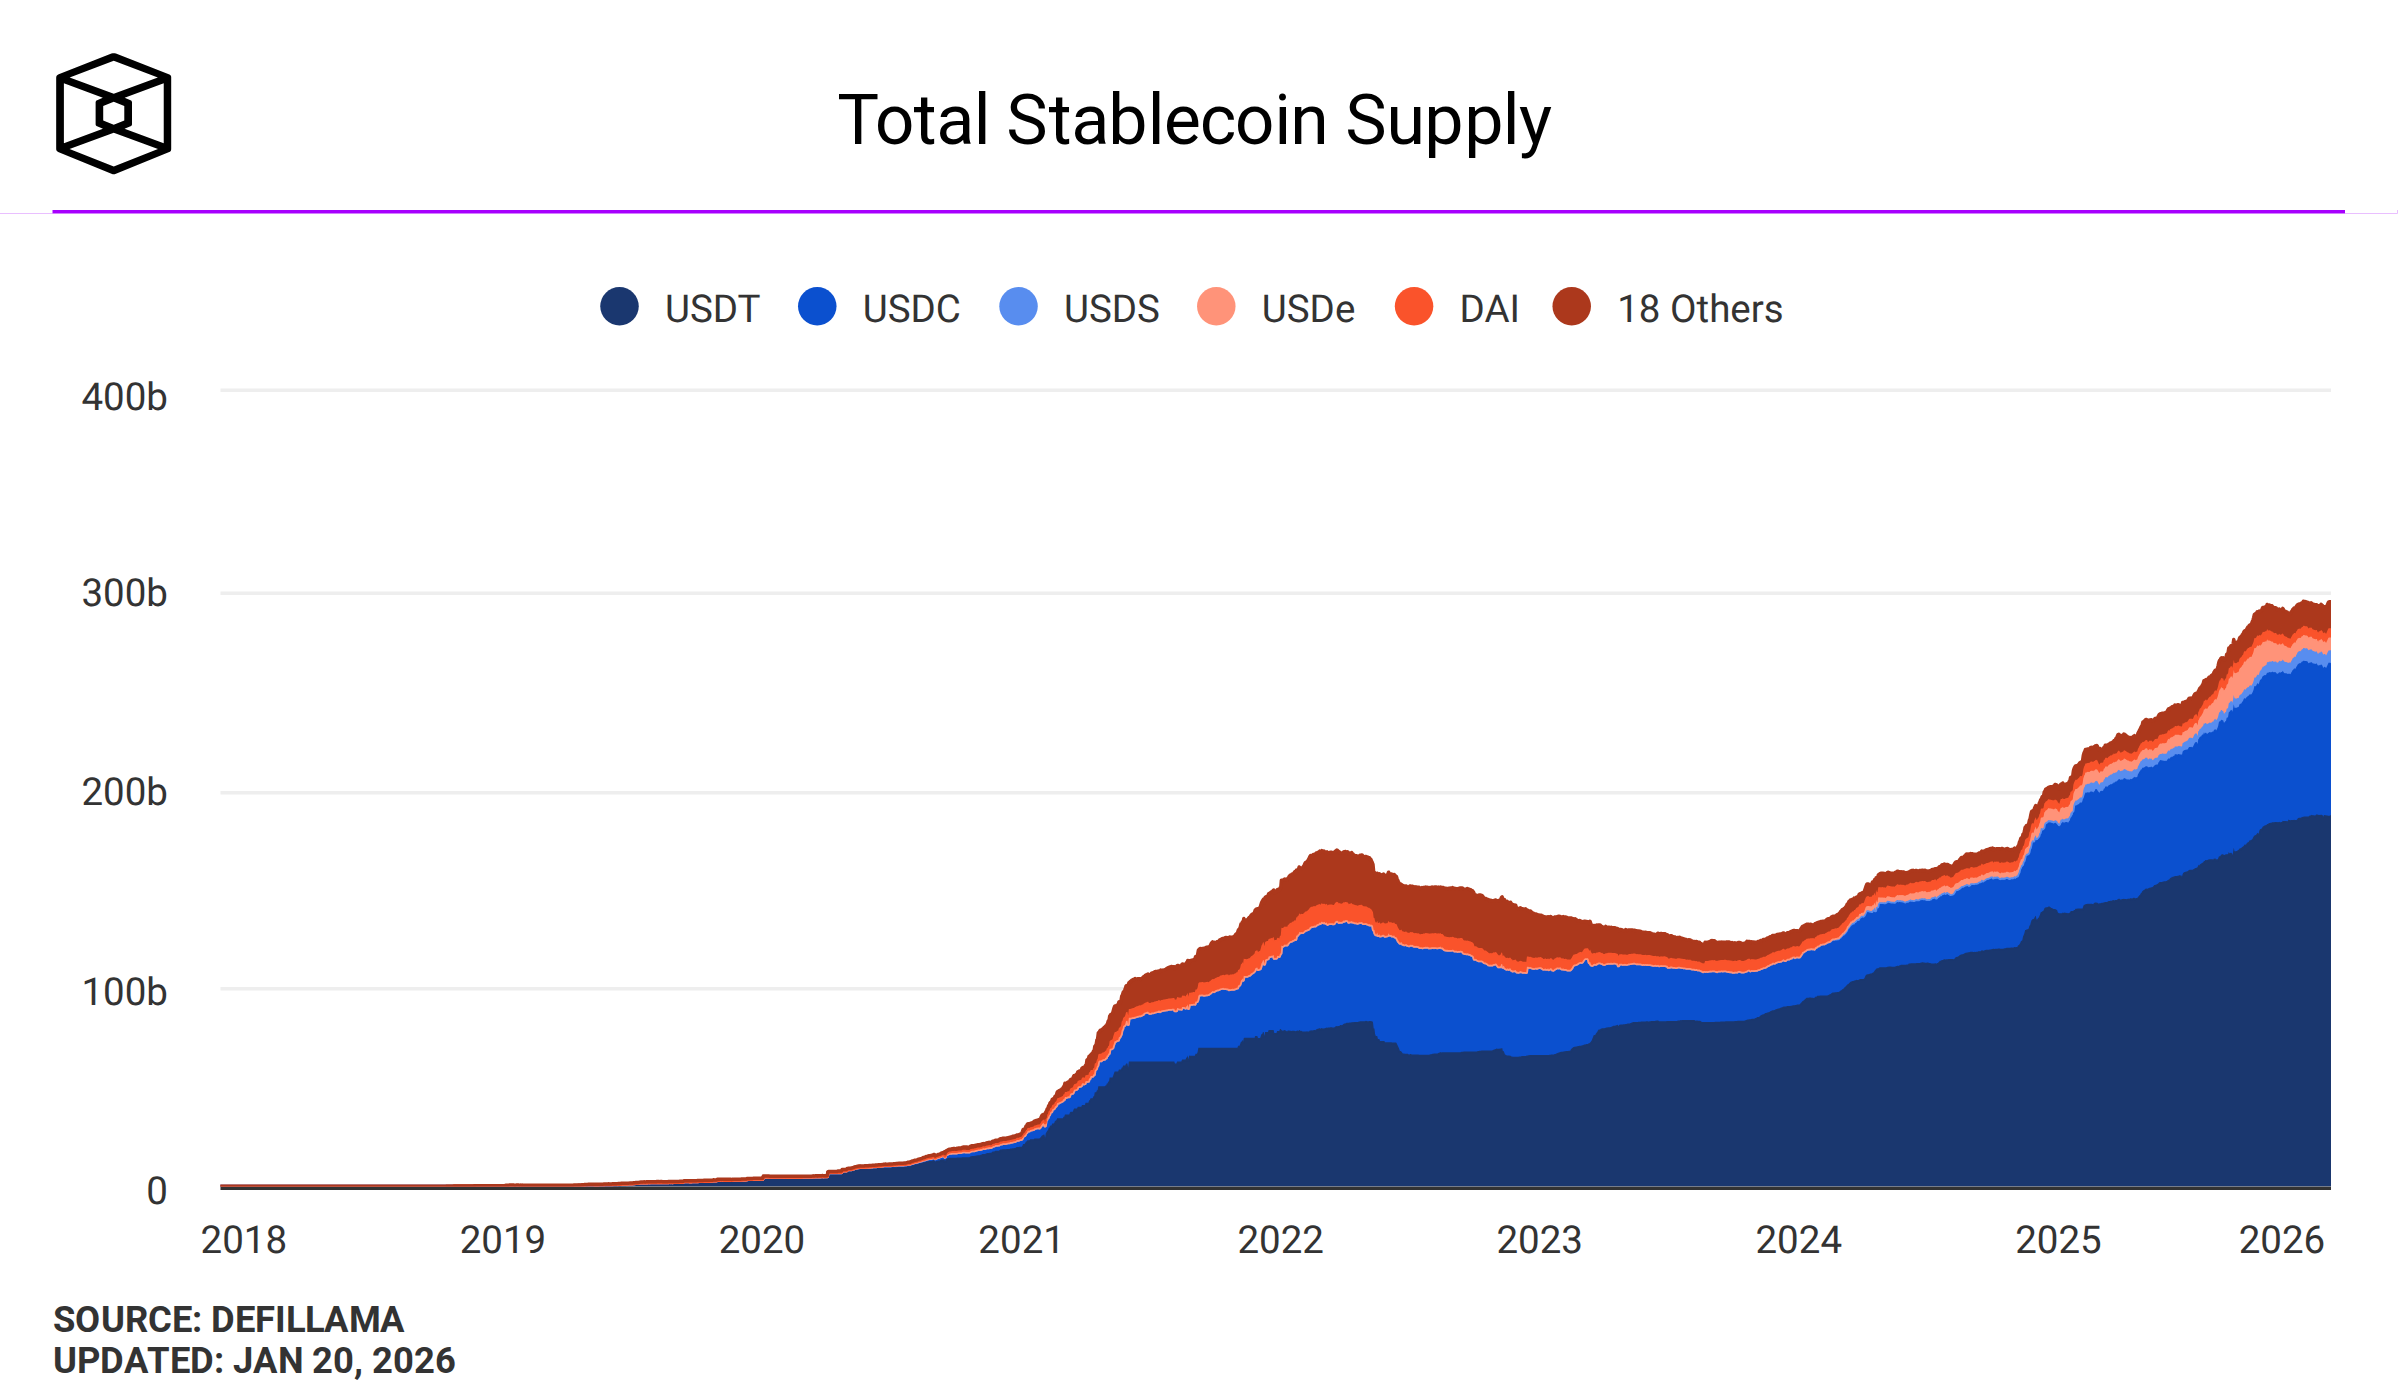
\includegraphics[width=.8\textwidth]{Figures/total-stablecoin-supply.png}
  \end{figure}
  \textbf{Dominant players}: Tether (USDT), USD Coin (USDC), and DAI.

  \vspace{0.5em}
  \textbf{What stablecoins are used for}:
  \begin{itemize}
    \item Trading pairs on exchanges (BTC/USDT instead of BTC/USD)
    \item DeFi collateral, lending, and liquidity provision
    \item Cross-border payments and remittances
  \end{itemize}
\end{frame}



\begin{frame}{Stablecoin Market Share}
  
  \textbf{Key observation}: The market is highly concentrated.
  
  \vspace{0.5em}
  \begin{itemize}
    \item USDT + USDC = $\approx$90\% of total stablecoin market cap
    \item Concentration \textit{increased} after Terra collapse (May 2022)
    \item Most trading volume flows through USDT
  \end{itemize}
  
  \vspace{1em}
  \textbf{Why this matters}:
  \begin{itemize}
    \item Systemic risk: Problems at Tether could affect entire crypto ecosystem
    \item Regulatory focus: Large stablecoins attract more scrutiny
    \item Network effects: Liquidity begets liquidity
  \end{itemize}
\end{frame}

%----------------------------------------------------------------------------------------
\section{Types of Stablecoins}
%----------------------------------------------------------------------------------------

\begin{frame}{Stablecoin Taxonomy}
  \begin{center}
  \resizebox{1\textwidth}{!}{\begin{tabular}{lll}
    \toprule
    \textbf{Type} & \textbf{Backing} & \textbf{Examples} \\
    \midrule
    Fiat-backed & USD in bank accounts, T-bills & USDT, USDC \\
    Crypto-backed & Cryptocurrency (over-collateralised) & DAI \\
    Algorithmic & No collateral; supply adjustments & UST (failed) \\
    Commodity-backed & Gold, other commodities & PAXG \\
    \bottomrule
  \end{tabular}}
  \end{center}
  
  \vspace{1em}
  \textbf{Key distinction}:
  \begin{itemize}
    \item \textbf{Off-chain collateral} (fiat, commodities): Requires trust in custodian
    \item \textbf{On-chain collateral} (crypto): Verifiable on blockchain, but volatile
    \item \textbf{No collateral} (algorithmic): Relies on mechanism design---fragile
  \end{itemize}
  
  \vspace{0.5em}
  We'll examine each type in detail.
\end{frame}

%----------------------------------------------------------------------------------------

\begin{frame}{Fiat-Backed Stablecoins}
\begin{center}
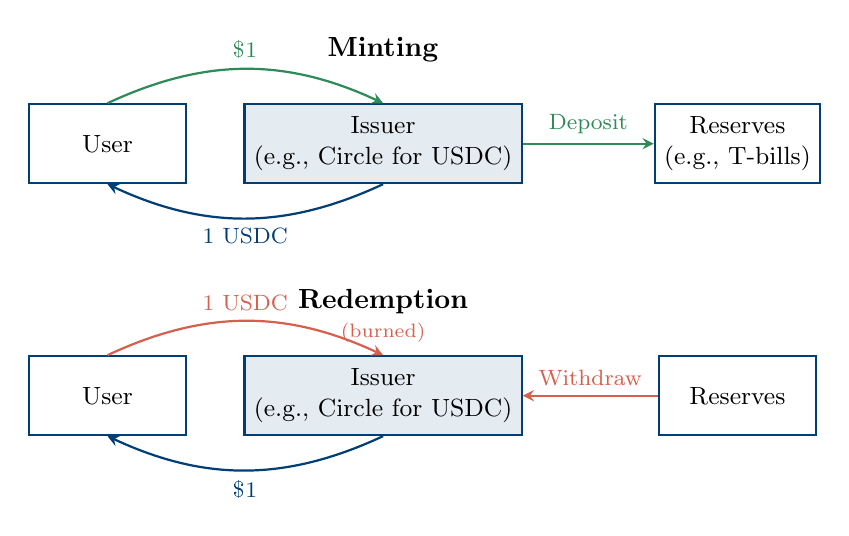
\begin{tikzpicture}[
    node distance=2.5cm,
    box/.style={rectangle, draw=ImperialBlue, fill=white, thick, minimum width=2cm, minimum height=1cm, align=center, font=\small},
    arrow/.style={->, thick, >=stealth},
    label/.style={font=\footnotesize, align=center}
]

% === MINTING ===
\node at (0, 2) {\textbf{Minting}};

\node[box] (user1) at (-3.5, 0.8) {User};
\node[box, fill=ImperialBlue!10] (issuer1) at (0, 0.8) {Issuer\\ (e.g., Circle for USDC)};
\node[box] (reserves1) at (4.5, 0.8) {Reserves\\ (e.g., T-bills)};

\draw[arrow, AccentGreen] (user1.north) to[bend left=25] node[above, label] {\$1} (issuer1.north);
\draw[arrow, AccentGreen] (issuer1) -- node[above, label] {Deposit} (reserves1);
\draw[arrow, ImperialBlue] (issuer1.south) to[bend left=25] node[below, label] {1 USDC} (user1.south);

% === REDEMPTION ===
\node at (0, -1.2) {\textbf{Redemption}};

\node[box] (user2) at (-3.5, -2.4) {User};
\node[box, fill=ImperialBlue!10] (issuer2) at (0, -2.4) {Issuer\\ (e.g., Circle for USDC)};
\node[box] (reserves2) at (4.5, -2.4) {Reserves};

\draw[arrow, AccentOrange] (user2.north) to[bend left=25] node[above, label] {1 USDC} (issuer2.north);
\draw[arrow, AccentOrange] (reserves2) -- node[above, label] {Withdraw} (issuer2);
\draw[arrow, ImperialBlue] (issuer2.south) to[bend left=25] node[below, label] {\$1} (user2.south);

\node[font=\scriptsize, AccentOrange] at (0, -1.6) {(burned)};

\end{tikzpicture}
\end{center}

\vspace{0.5em}
\textbf{The peg is maintained by arbitrage}:
\begin{itemize}
  \item If market price $>$ \$1: Mint new coins, sell on market, profit
  \item If market price $<$ \$1: Buy on market, redeem for \$1, profit
\end{itemize}
\end{frame}

\begin{frame}{Tether (USDT): The Dominant Stablecoin}
  % [FIGURE 4: USDT market cap over time]
  % Source: CoinGecko or Tether transparency page
  
  \textbf{The basics}:
  \begin{itemize}
    \item Launched in 2014; the largest stablecoin by far ($>$\$150bn)
    \item Issued by Tether Limited (related to Bitfinex exchange)
    \item Claims 1:1 backing by reserves
  \end{itemize}
  
  \vspace{1em}
  \textbf{The controversies}:
  \begin{itemize}
    \item \textbf{No full audit}: Only ``attestations'' (point-in-time snapshots), not comprehensive audits
    \item \textbf{Reserve quality}: Previously held commercial paper, now mostly T-bills
    \item \textbf{Bitfinex relationship}: \$850M loan to cover Bitfinex losses (revealed 2019)
    \item \textbf{Regulatory settlements}: Paid \$41M to CFTC (2021) for misrepresenting reserves
  \end{itemize}
  
  \vspace{0.5em}
  Despite controversies, USDT has maintained its peg through multiple crises.
\end{frame}

\begin{frame}{Tether Reserve Composition}
  % [FIGURE 5: Tether reserve breakdown pie chart - current data]
  % Source: Tether transparency page (tether.to/en/transparency)
  
  \textbf{Current reserves} (2024):
  \begin{itemize}
    \item $\approx$80\% US Treasury bills
    \item $\approx$12\% Secured loans
    \item $\approx$5\% Bitcoin and precious metals
    \item $\approx$3\% Other investments
  \end{itemize}
  
  \vspace{1em}
  \textbf{Evolution}: Tether has shifted toward safer assets after criticism.
  \begin{itemize}
    \item 2021: $\approx$50\% commercial paper (risky corporate debt)
    \item 2024: Mostly T-bills (much safer)
  \end{itemize}
  
  \vspace{0.5em}
  \textbf{The trust problem}: Users must trust Tether's self-reported numbers. Without a full audit, reserve claims cannot be independently verified.
\end{frame}

\begin{frame}{USD Coin (USDC): The ``Transparent'' Alternative}
  \textbf{The basics}:
  \begin{itemize}
    \item Launched 2018 by Circle (in partnership with Coinbase)
    \item Second largest stablecoin ($\approx$\$70bn)
    \item Positioned as the regulated, transparent option
  \end{itemize}
  
  \vspace{0.5em}
  \textbf{Key differences from USDT}:
  \begin{itemize}
    \item Monthly attestations from Big Four accounting firm (Grant Thornton, now Deloitte)
    \item Reserves held in regulated US financial institutions
    \item Circle is a licensed money transmitter
    \item More detailed reserve disclosures
  \end{itemize}
  
  \vspace{1em}
  \textbf{Reserve composition} (2024):
  \begin{itemize}
    \item $\approx$80\% short-dated US Treasuries
    \item $\approx$20\% cash at regulated banks
  \end{itemize}
  
  \vspace{0.5em}
  USDC was seen as ``safer''---until March 2023.
\end{frame}

\begin{frame}{Case Study: The USDC Depeg (March 2023)}
  % [FIGURE 6: USDC price chart March 10-13, 2023 showing drop to $0.87]
  % Source: CoinGecko, TradingView
  
  \textbf{What happened}:
  \begin{itemize}
    \item March 10, 2023: Silicon Valley Bank (SVB) collapses
    \item Circle reveals \$3.3 billion of USDC reserves ($\approx$8\%) held at SVB
    \item Panic: Will Circle be able to redeem at \$1?
    \item USDC drops to \highlight{\$0.87} on some exchanges
  \end{itemize}
  
  \vspace{0.5em}
  \textbf{The resolution}:
  \begin{itemize}
    \item March 12: US government guarantees all SVB deposits
    \item Circle confirms full access to SVB funds
    \item USDC returns to \$1 peg within 48 hours
  \end{itemize}
  
  \vspace{0.5em}
  \textbf{Lessons}:
  \begin{itemize}
    \item Even ``safe'' stablecoins face bank counterparty risk
    \item Transparency helped: Circle disclosed exposure quickly
    \item Government backstop restored confidence
  \end{itemize}
\end{frame}

\begin{frame}{Fiat-Backed Stablecoins: The Bank Run Problem}
\begin{center}
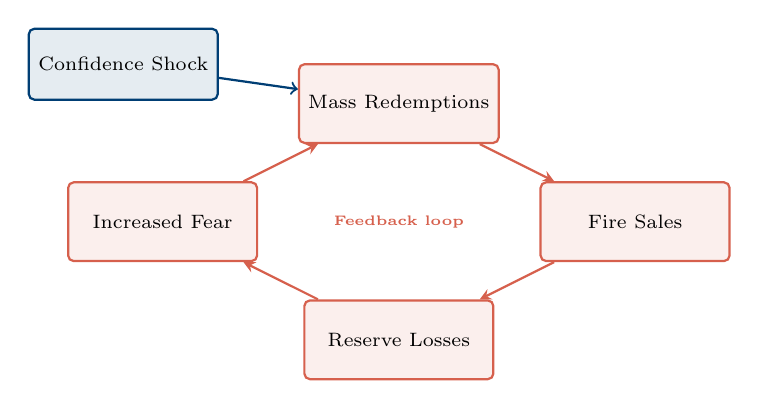
\begin{tikzpicture}[
    node distance=2cm,
    box/.style={rectangle, draw=AccentOrange, fill=AccentOrange!10, thick, minimum width=2.4cm, minimum height=1cm, align=center, font=\scriptsize, rounded corners=2pt},
    trigger/.style={rectangle, draw=ImperialBlue, fill=ImperialBlue!10, thick, minimum width=2.4cm, minimum height=0.9cm, align=center, font=\scriptsize, rounded corners=2pt},
    arrow/.style={->, thick, >=stealth, AccentOrange},
    label/.style={font=\tiny, align=center}
]

% Trigger
\node[trigger] (trigger) at (-3.5, 1) {Confidence Shock};

% Cycle nodes
\node[box] (redeem) at (0, 0.5) {Mass Redemptions};
\node[box] (sell) at (3, -1) {Fire Sales};
\node[box] (loss) at (0, -2.5) {Reserve Losses};
\node[box] (fear) at (-3, -1) {Increased Fear};

% Arrows
\draw[->, thick, ImperialBlue] (trigger) -- (redeem);
\draw[arrow] (redeem) -- (sell);
\draw[arrow] (sell) -- (loss);
\draw[arrow] (loss) -- (fear);
\draw[arrow] (fear) -- (redeem);

% Center label
\node[font=\tiny, AccentOrange] at (0, -1) {\textbf{Feedback loop}};

\end{tikzpicture}
\end{center}

Fiat-backed stablecoins face the same run dynamics as traditional banks. \textbf{Key difference}: No deposit insurance, no backstop.

\vspace{0.5em}
\textbf{Mitigants}:
\begin{itemize}
  \item Hold only safest, most liquid assets (T-bills)
  \item Maintain reserves $\geq$ 100\% of issued stablecoins
  \item Redemption gates during stress (controversial)
\end{itemize}
\end{frame}


%----------------------------------------------------------------------------------------

\begin{frame}{Crypto-Backed Stablecoins}

\textbf{Crypto-Backed Stablecoins:} Collateral in the form of other cryptocurrencies. 
\vspace{0.5em}

  \textbf{Problem}: If collateral is volatile crypto, how do you maintain a \$1 peg?
  
  \vspace{0.5em}
  \textbf{Solution}: Require \textit{more} collateral than the stablecoins issued.
  
  \vspace{1em}
  \textbf{Example}: To mint \$100 of stablecoins, deposit \$150 of ETH.
  \begin{itemize}
    \item If ETH drops 20\%, collateral is still worth \$120
    \item Stablecoins remain fully backed
    \item If collateral drops too far, it gets liquidated
  \end{itemize}
  
  \vspace{1em}
  \textbf{Trade-off}:
  \begin{itemize}
    \item \good{Transparent}: Collateral is on-chain, verifiable
    \item \good{No bank counterparty risk}
    \item \bad{Capital inefficient}: Need \$150 to create \$100
    \item \bad{Inherits crypto volatility risks}
  \end{itemize}
\end{frame}

\begin{frame}{DAI: The Leading Crypto-Backed Stablecoin}
  % [FIGURE 8: DAI market cap and peg stability over time]
  % Source: DeFiLlama, CoinGecko

  \begin{figure}
    \centering
    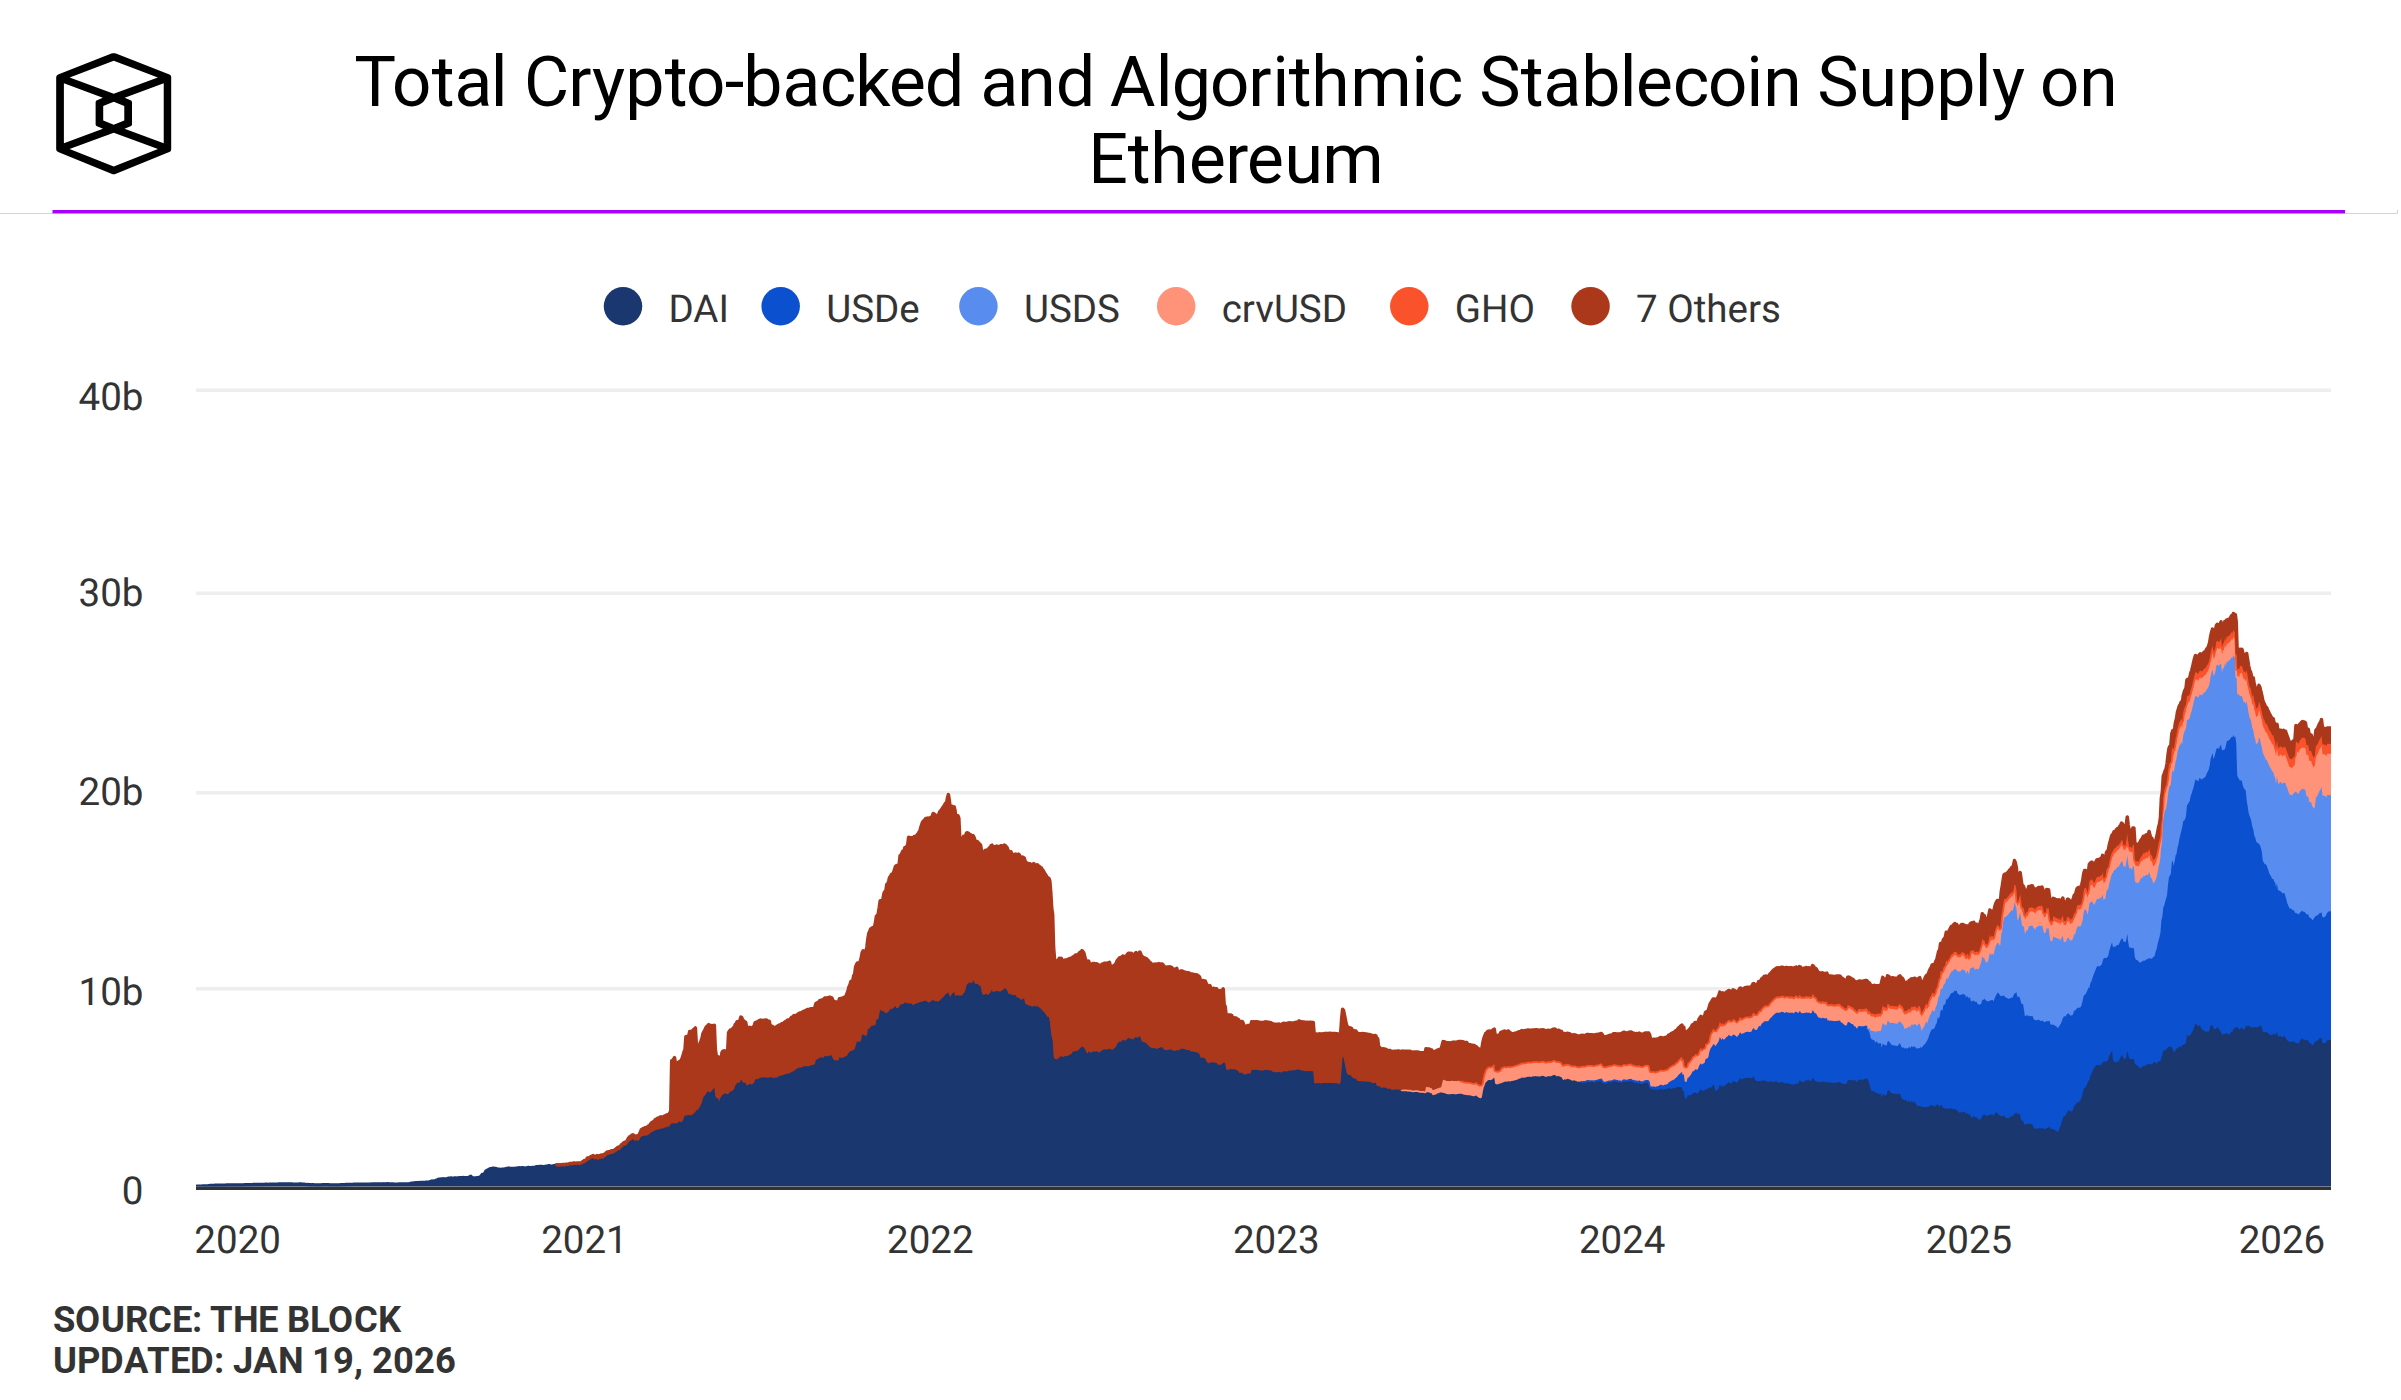
\includegraphics[width=.8\textwidth]{Figures/total-crypto-backed-and-algorithmic-stablecoin-supply.png}
  \end{figure}
  
  \textbf{The basics}:
  \begin{itemize}
    \item Launched 2017 by MakerDAO
    \item Decentralised: No single company controls it
    \item DAI is essentially a loan against your crypto (i.e., DeFi lending)
  \end{itemize}

\end{frame}

\begin{frame}{DAI: Collateralisation and Liquidation}
  \textbf{Example}: You deposit 1 ETH (worth \$3,000) as collateral.
    \begin{itemize}
    \item Minimum collateralisation ratio: 150\%
    \item Maximum DAI you can mint: \$3,000 / 1.5 = \$2,000
    \item You mint \$1,500 DAI (200\% collateralisation, safer)
  \end{itemize}
  
  \vspace{1em}
  \textbf{If ETH drops to \$2,000}:
  \begin{itemize}
    \item Your collateral ratio: \$2,000 / \$1,500 = 133\%
    \item Below 150\% threshold $\rightarrow$ \highlight{Liquidation risk}
    \item Liquidators can repay part of your debt and seize collateral at a discount
  \end{itemize}
  
  \vspace{1em}
  \textbf{Why this maintains the peg}:
  \begin{itemize}
    \item DAI is always backed by $>$100\% collateral value
    \item Liquidations ensure undercollateralised positions are closed
    \item If DAI $<$ \$1: Cheaper to repay debt, reducing supply
    \item If DAI $>$ \$1: Profitable to mint more, increasing supply
  \end{itemize}
\end{frame}

\begin{frame}{DAI Collateral Composition}
  % [FIGURE 9: DAI collateral breakdown - pie chart showing ETH, USDC, stETH, etc.]
  % Source: DaiStats.com, MakerBurn.com
  
  \textbf{Evolution}: DAI was originally backed only by ETH. Now accepts multiple collateral types:
  
  \vspace{0.5em}
  \begin{itemize}
    \item ETH and wrapped ETH variants ($\approx$40\%)
    \item USDC and other stablecoins ($\approx$30\%)
    \item Real-world assets (emerging category)
    \item Other approved tokens
  \end{itemize}
  
  \vspace{1em}
  \textbf{The USDC controversy}:
  \begin{itemize}
    \item DAI claims to be ``decentralised''
    \item But $\approx$30\% backed by USDC (centralised, can freeze addresses)
    \item During March 2023 USDC depeg, DAI also dropped briefly
    \item Tension between stability and decentralisation
  \end{itemize}
\end{frame}

%----------------------------------------------------------------------------------------

\begin{frame}{Algorithmic Stablecoins}
  \textbf{Idea}: Maintain the peg through supply adjustments, not collateral.
  
  \vspace{1em}
  \textbf{If price $>$ \$1}: Increase supply (mint new coins) $\rightarrow$ price falls
  
  \textbf{If price $<$ \$1}: Decrease supply (remove coins) $\rightarrow$ price rises
  
  \vspace{1em}
  \textbf{The challenge}: Increasing supply is easy. How do you \textit{decrease} supply?
  
  \vspace{1em}
  \textbf{Common mechanisms}:
  \begin{itemize}
    \item \textbf{Seigniorage shares}: Issue ``bonds'' that promise future stablecoins
    \item \textbf{Dual-token}: Absorb volatility into a second token
    \item \textbf{Rebase}: Automatically adjust everyone's balances
  \end{itemize}
  
  \vspace{1em}
  All of these require \highlight{continued confidence} in the system. If confidence breaks, there's no collateral to fall back on.
\end{frame}

\begin{frame}{Terra/Luna: Anatomy of a Collapse}
  % [FIGURE 10: UST and LUNA price during May 2022 collapse]
  % Source: CoinGecko, TradingView
  
  \textbf{The mechanism} (simplified):
  \begin{itemize}
    \item UST (stablecoin) paired with LUNA (volatile token)
    \item To mint 1 UST: Burn \$1 worth of LUNA
    \item To redeem 1 UST: Burn UST, receive \$1 worth of LUNA
    \item Arbitrage should maintain the peg
  \end{itemize}
  
  \vspace{1em}
  \textbf{The sweetener}: Anchor protocol paid \highlight{20\% APY} on UST deposits.
  
  \vspace{1em}
  \textbf{At peak} (April 2022):
  \begin{itemize}
    \item UST market cap: $\approx$\$18 billion
    \item LUNA market cap: $\approx$\$40 billion
    \item LUNA price: $\approx$\$80
  \end{itemize}
\end{frame}

\begin{frame}{The Death Spiral (May 2022)}
  % [FIGURE 11: LUNA supply explosion chart during collapse]
  % Source: On-chain data, Messari
  
  \textbf{May 7-13, 2022}:
  \begin{enumerate}
    \item Large UST withdrawals from Anchor (confidence shock)
    \item UST drops slightly below \$1
    \item Holders redeem UST for LUNA (minting new LUNA)
    \item LUNA supply increases $\rightarrow$ LUNA price falls
    \item Now \$1 of LUNA is worth less $\rightarrow$ need more LUNA per UST redeemed
    \item LUNA supply explodes: 350 million $\rightarrow$ 6.5 \textit{trillion}
    \item LUNA price: \$80 $\rightarrow$ \$0.0001
    \item With LUNA worthless, UST has no redemption value
    \item UST collapses to \$0.10
  \end{enumerate}
  
  \vspace{0.5em}
  \textbf{Total losses}: $\approx$\$60 billion in value destroyed in one week.
\end{frame}

\begin{frame}{Why Algorithmic Stablecoins Are Fragile}
  % [FIGURE 12: Diagram showing reflexive death spiral feedback loop]
  % Can create in TikZ
  
  \textbf{The fundamental problem}: Circular backing.
  
  \vspace{0.5em}
  \begin{itemize}
    \item UST's value depends on ability to redeem for LUNA
    \item LUNA's value depends on demand for UST
    \item If one loses confidence, both collapse
  \end{itemize}
  
  \vspace{1em}
  \textbf{Contrast with fiat-backed}:
  \begin{itemize}
    \item USDC is backed by T-bills
    \item T-bills have value independent of USDC demand
    \item External collateral breaks the reflexivity
  \end{itemize}
  
  \vspace{1em}
  \textbf{Lesson}: Algorithmic stablecoins can work during good times. The question is whether they survive bad times. Terra didn't.
  
  \vspace{0.5em}
  No algorithmic stablecoin has achieved both scale and long-term stability.
\end{frame}

%----------------------------------------------------------------------------------------
\section{Stablecoin Risks and Regulation}
%----------------------------------------------------------------------------------------

\begin{frame}{Summary of Stablecoin Risks}
  \begin{center}
  \resizebox{1\textwidth}{!}{\begin{tabular}{ll}
    \toprule
    \textbf{Risk} & \textbf{Description} \\
    \midrule
    Run risk & Mass redemptions exhaust reserves \\
    Reserve quality & Illiquid or risky assets can't meet redemptions \\
    Counterparty risk & Bank failures, custodian problems \\
    Operational risk & Smart contract bugs, key management \\
    Concentration & Few stablecoins dominate; failure is systemic \\
    Regulatory & Legal status unclear; potential bans or restrictions \\
    \bottomrule
  \end{tabular}}
  \end{center}
  
  \vspace{1em}
  \textbf{Systemic concern}: Stablecoins are deeply embedded in crypto markets. A major stablecoin failure could trigger cascading liquidations across DeFi.
\end{frame}

\begin{frame}{Regulatory Landscape: Europe (MiCA)}
  % [FIGURE 13: MiCA timeline or key requirements infographic]
  % Source: European Commission, create summary graphic
  
  The EU's \highlight{Markets in Crypto-Assets Regulation} (MiCA) came into force in 2024.
  
  \vspace{1em}
  \textbf{Key requirements for stablecoin issuers}:
  \begin{itemize}
    \item Must be authorised as an electronic money institution
    \item Reserves must be 1:1 and held in secure, liquid assets
    \item Regular audits and public disclosures required
    \item Significant stablecoins face stricter capital requirements
    \item Issuers must have EU presence
  \end{itemize}
  
  \vspace{1em}
  \textbf{Impact}:
  \begin{itemize}
    \item Tether (USDT) delisted from some EU exchanges
    \item USDC pursuing MiCA compliance
    \item Creates regulatory clarity but raises compliance costs
  \end{itemize}
\end{frame}

\begin{frame}{Regulatory Landscape: Europe (MiCA)}
  \begin{figure}
    \centering
    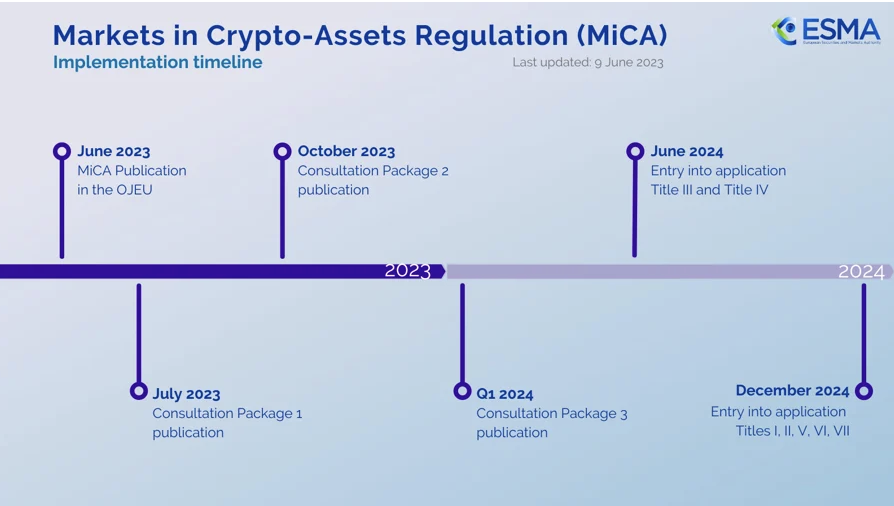
\includegraphics[width=1\textwidth]{Figures/MiCA timeline.png}
  \end{figure}
\end{frame}


\begin{frame}{Regulatory Landscape: United States}
  \textbf{Current state}: Fragmented, no comprehensive stablecoin law.
  
  \vspace{1em}
  \textbf{Key developments}:
  \begin{itemize}
    \item SEC: Some stablecoins may be securities
    \item CFTC: Enforcement actions against Tether
    \item OCC: National banks can hold stablecoin reserves
    \item Congress: Multiple stablecoin bills proposed, none passed
  \end{itemize}
  
  \vspace{1em}
  \textbf{Proposed requirements} (various bills):
  \begin{itemize}
    \item 1:1 reserve backing in high-quality liquid assets
    \item Bank-like regulatory oversight
    \item Regular examinations and disclosures
    \item Potential Fed approval for large issuers
  \end{itemize}
  
  \vspace{0.5em}
  \textbf{Uncertainty}: Regulatory approach depends heavily on political landscape and may shift significantly.
\end{frame}

\begin{frame}{Stablecoins vs Traditional Payment Systems}
  % [FIGURE 14: Comparison chart - settlement times, costs, availability]
  % Can create as a table or bar chart
  
  \begin{center}
  \resizebox{1\textwidth}{!}{\begin{tabular}{lccc}
    \toprule
    & \textbf{Wire Transfer} & \textbf{Card Payment} & \textbf{Stablecoin} \\
    \midrule
    Settlement & 1-3 days & 1-2 days & Minutes \\
    Availability & Business hours & 24/7 & 24/7 \\
    Cross-border & Expensive & Fees apply & Low cost \\
    Access & Bank account & Card issuer & Wallet only \\
    Reversibility & Possible & Chargebacks & Generally not \\
    \bottomrule
  \end{tabular}}
  \end{center}
  
  \vspace{1em}
  \textbf{Stablecoin advantages}: Speed, availability, programmability
  
  \textbf{Stablecoin disadvantages}: No consumer protections, regulatory uncertainty, counterparty risks
  
  \vspace{0.5em}
  For some use cases (remittances, DeFi), stablecoins offer clear benefits. For everyday consumer payments, traditional systems may be preferable.
\end{frame}

%----------------------------------------------------------------------------------------
\section{Central Bank Digital Currencies (CBDCs)}
%----------------------------------------------------------------------------------------

\begin{frame}{What is a CBDC?}
  \begin{block}{Central Bank Digital Currency}
    A digital form of central bank money, denominated in the national currency and issued as a direct liability of the central bank.
  \end{block}
  
  \vspace{1em}
  \textbf{How it differs from}:
  \begin{itemize}
    \item \textbf{Physical cash}: Digital, not physical
    \item \textbf{Bank deposits}: Direct central bank liability, not commercial bank
    \item \textbf{Stablecoins}: Issued by government, not private company
    \item \textbf{Bitcoin}: Centralised issuance, not decentralised
  \end{itemize}
  
  \vspace{1em}
  \textbf{Key point}: A CBDC would give citizens direct access to central bank money in digital form---something currently only banks have.
\end{frame}

\begin{frame}{Retail vs Wholesale CBDCs}
  % [FIGURE 15: Diagram showing retail CBDC (central bank → public) vs wholesale (central bank → banks)]
  % Can create in TikZ
  
  \textbf{Retail CBDC}: Available to households and businesses
  \begin{itemize}
    \item Used for everyday transactions
    \item Competes with cash and bank deposits
    \item Examples: Digital Yuan (China), Sand Dollar (Bahamas)
  \end{itemize}
  
  \vspace{1em}
  \textbf{Wholesale CBDC}: Available only to financial institutions
  \begin{itemize}
    \item Used for interbank settlements
    \item Competes with existing reserve systems
    \item Examples: Project Helvetia (Switzerland), various pilots
  \end{itemize}
  
  \vspace{1em}
  Most public discussion focuses on \highlight{retail CBDCs}---these raise the most significant policy questions.
\end{frame}

\begin{frame}{CBDC Design Choices}
  % [FIGURE 16: 2x2 matrix showing design choices]
  % Can create in TikZ or as a table
  
  \textbf{Key design decisions}:
  \vspace{-1em}
  \begin{center}
  \resizebox{1\textwidth}{!}{\begin{tabular}{lll}
    \toprule
    \textbf{Choice} & \textbf{Option A} & \textbf{Option B} \\
    \midrule
    Architecture & Direct (CB manages accounts) & Intermediated (banks distribute) \\
    Technology & Account-based (identity) & Token-based (possession) \\
    Interest & Interest-bearing & Non-interest-bearing \\
    Privacy & Anonymous (like cash) & Traceable (like deposits) \\
    Limits & Unlimited holdings & Capped holdings \\
    \bottomrule
  \end{tabular}}
  \end{center}
  
  \vspace{0.5em}
  Most proposed CBDCs are \textbf{intermediated} (banks handle distribution) and \textbf{non-anonymous} (transactions traceable).
\end{frame}


\begin{frame}{Global CBDC Development}
  \begin{figure}
    \centering
    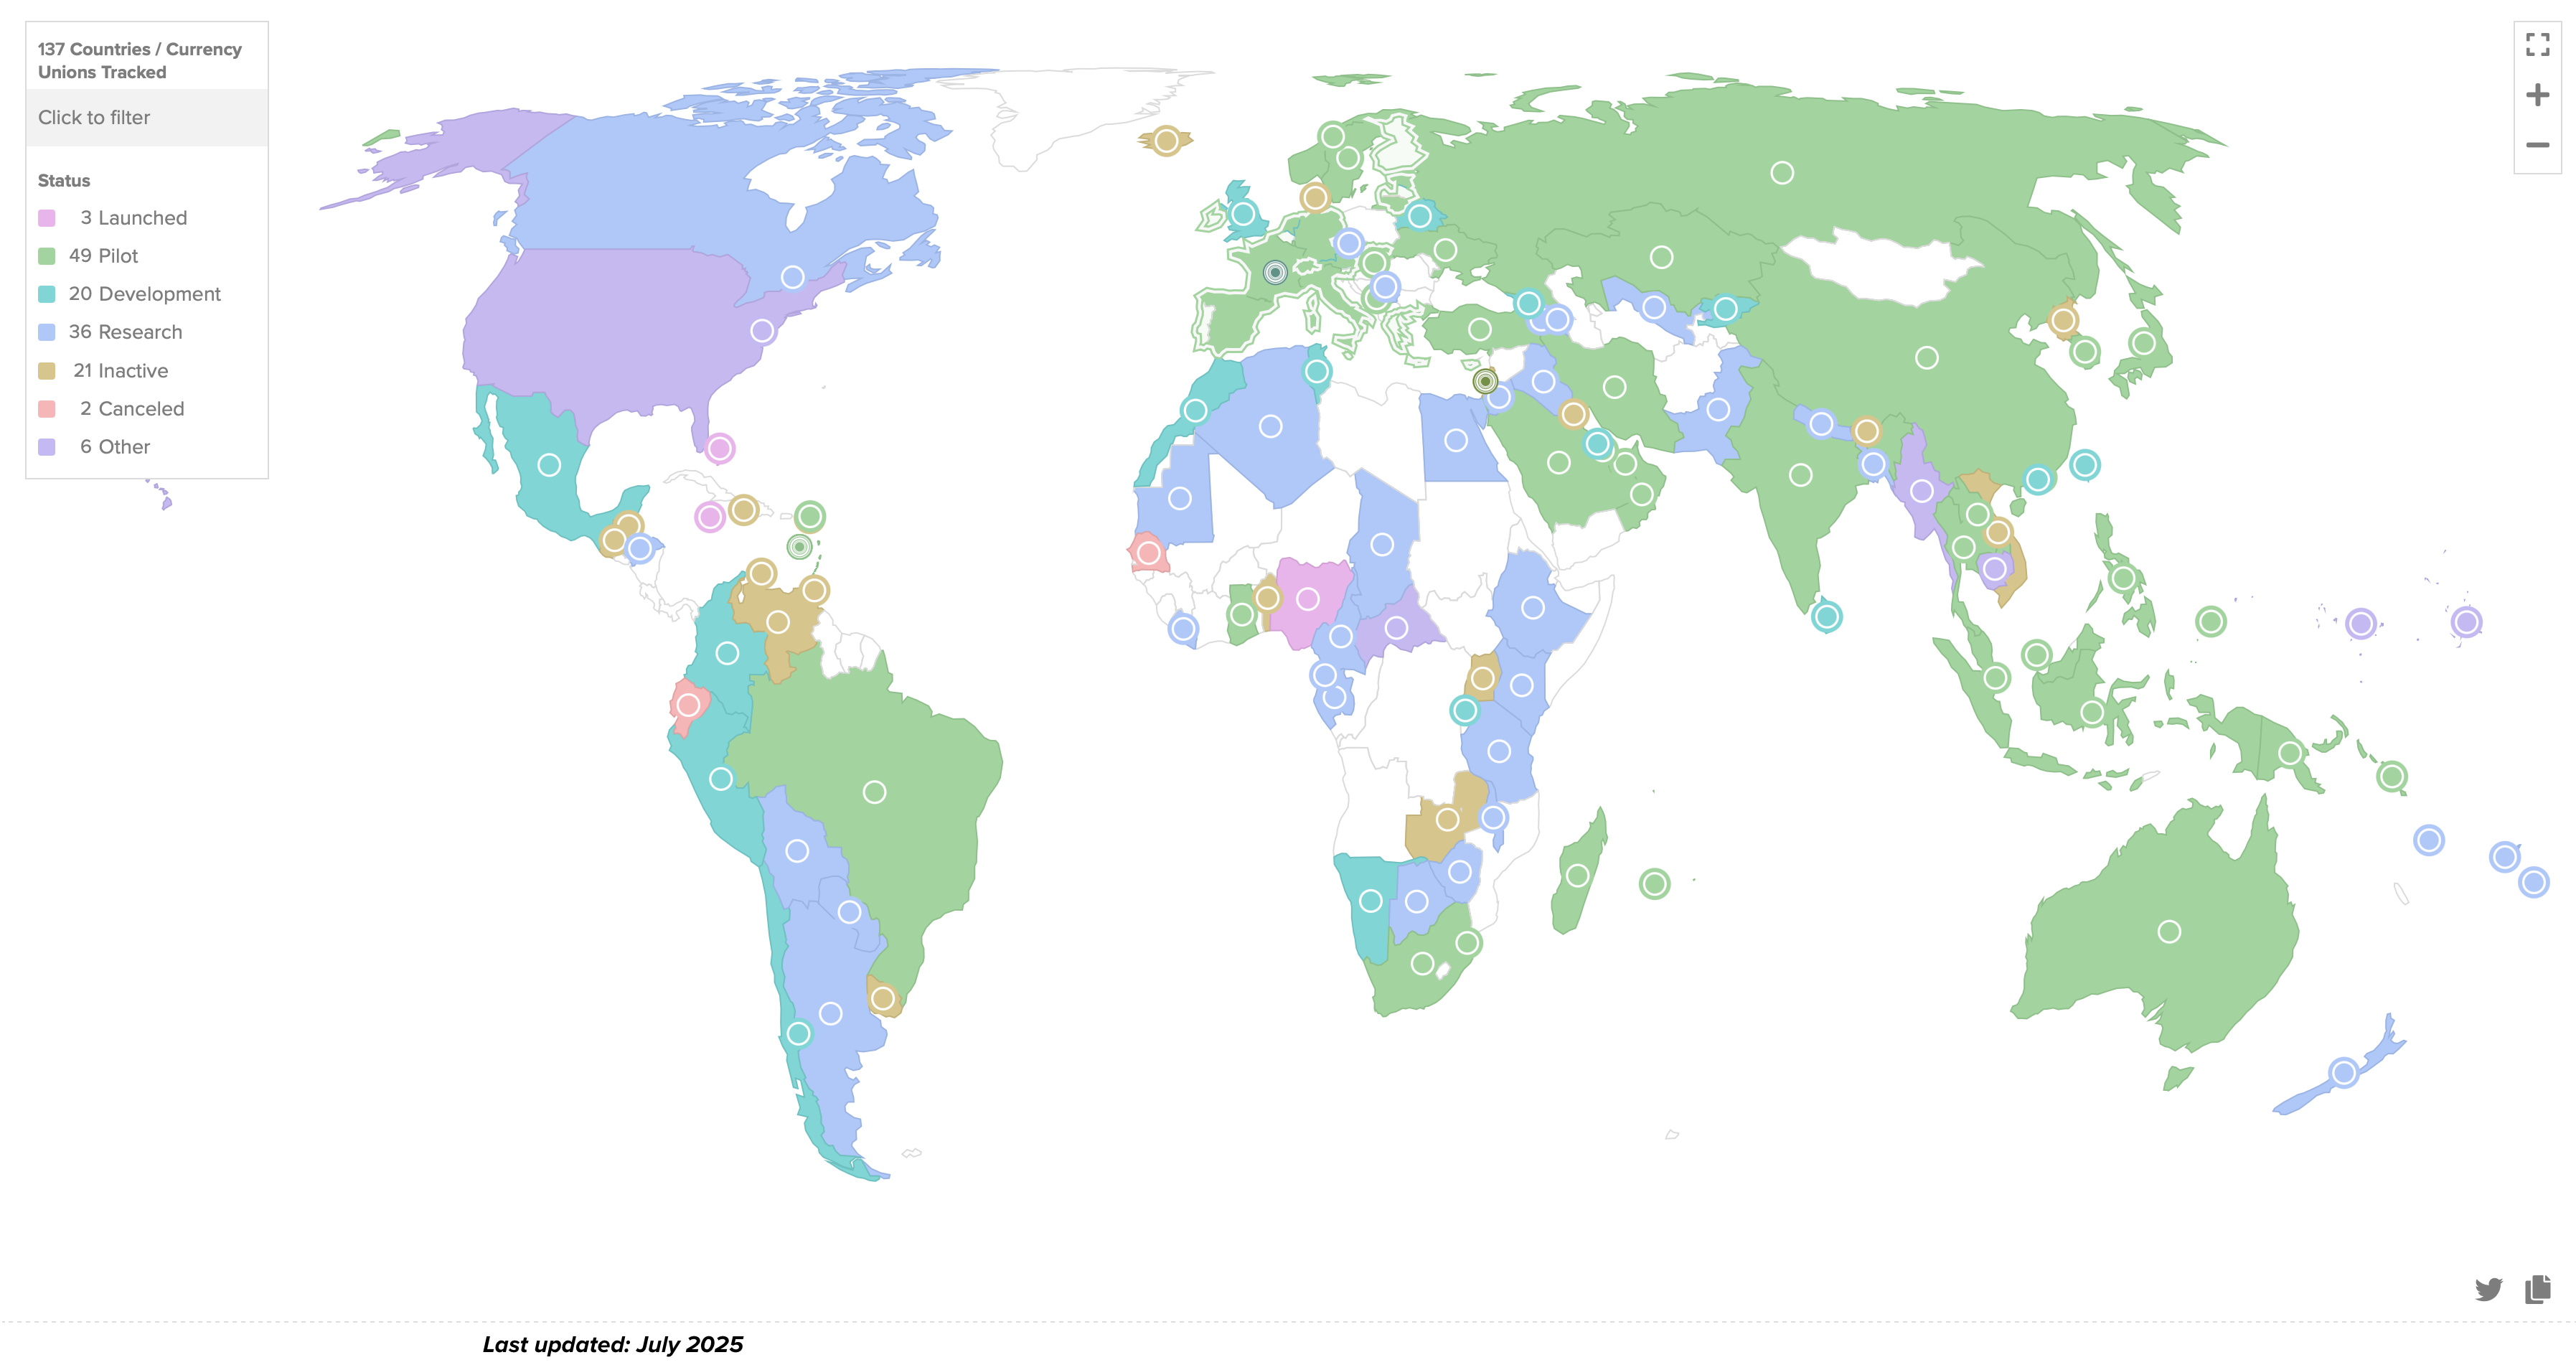
\includegraphics[width=1\textwidth]{Figures/CBDC status.png}
    \\[0.3em]\footnotesize Source: \url{https://www.atlanticcouncil.org/cbdctracker/}
  \end{figure}
\end{frame}

\begin{frame}{Why Are Central Banks Interested?}
  % [FIGURE 17: BIS survey - motivations by AE vs EMDE]
  % Source: BIS CBDC surveys (you have this figure)
  
  \textbf{Advanced economies}:
  \begin{itemize}
    \item Payment system resilience and efficiency
    \item Declining cash usage (especially Nordics)
    \item Respond to private stablecoins
    \item Maintain monetary sovereignty
  \end{itemize}
  
  \vspace{1em}
  \textbf{Emerging economies}:
  \begin{itemize}
    \item Financial inclusion (unbanked populations)
    \item Reduce cash handling costs
    \item Combat informal economy
    \item Improve cross-border payments
  \end{itemize}
  
  \vspace{0.5em}
  Different motivations lead to different designs.
\end{frame}

%----------------------------------------------------------------------------------------
\section{CBDC Trade-offs}
%----------------------------------------------------------------------------------------

\begin{frame}{The Bank Disintermediation Problem}
  % [FIGURE 19: Diagram showing deposits flowing from banks to CBDC]
  % Can create in TikZ
  
  \textbf{The concern}: If citizens can hold money directly at the central bank, why keep deposits at commercial banks?
  
  \vspace{1em}
  \textbf{Potential consequences}:
  \begin{itemize}
    \item Deposits flow from banks to CBDC
    \item Banks lose cheap funding source
    \item Banks must rely on wholesale funding (more expensive)
    \item Credit availability may decrease
    \item During crises, ``digital bank runs'' could be instantaneous
  \end{itemize}
  
  \vspace{1em}
  \textbf{Proposed mitigants}:
  \begin{itemize}
    \item Cap CBDC holdings (e.g., €3,000 per person---ECB proposal)
    \item Make CBDC non-interest-bearing (less attractive than deposits)
    \item Tiered remuneration (penalty rate above threshold)
  \end{itemize}
\end{frame}

\begin{frame}{Privacy vs Surveillance}
  \textbf{The tension}: CBDCs could offer cash-like privacy or enable unprecedented surveillance.
  
  \vspace{1em}
  \textbf{Privacy advocates worry}:
  \begin{itemize}
    \item Every transaction could be tracked by the state
    \item Spending patterns reveal sensitive information
    \item Potential for political targeting or social control
    \item ``Programmable money'' could restrict what you buy
  \end{itemize}
  
  \vspace{1em}
  \textbf{Authorities argue}:
  \begin{itemize}
    \item Traceability needed for anti-money laundering (AML)
    \item Tax compliance requires some visibility
    \item Anonymity enables illicit finance
    \item Can design tiered privacy (anonymous for small amounts)
  \end{itemize}
  
  \vspace{0.5em}
  Design choices here reflect fundamental values about the state-citizen relationship.
\end{frame}

\begin{frame}{Monetary Policy Implications}
  \textbf{New tools}:
  \begin{itemize}
    \item \textbf{Direct transmission}: Interest on CBDC goes straight to public
    \item \textbf{Negative rates}: Could charge for holding CBDC (harder with cash)
    \item \textbf{Helicopter money}: Direct transfers to citizens
    \item \textbf{Programmability}: Time-limited spending vouchers
  \end{itemize}
  
  \vspace{1em}
  \textbf{Concerns}:
  \begin{itemize}
    \item Do we want central banks to have these powers?
    \item Negative rates on CBDC could be deeply unpopular
    \item Programmable restrictions raise civil liberties questions
    \item Expiring money could face legal challenges
  \end{itemize}
  
  \vspace{1em}
  CBDCs don't require these features, but they make them technically possible.
\end{frame}

\begin{frame}{CBDCs vs Stablecoins: A Comparison}
  \begin{center}
  \begin{tabular}{lll}
    \toprule
    & \textbf{Stablecoins} & \textbf{CBDCs} \\
    \midrule
    Issuer & Private companies & Central bank \\
    Backing & Reserves (varies) & Full faith of government \\
    Regulation & Evolving & Government-controlled \\
    Privacy & Pseudonymous & Design-dependent \\
    Innovation & Rapid & Slow, deliberate \\
    Interoperability & Cross-chain possible & Domestic focus \\
    Risk & Issuer default & Political risk \\
    \bottomrule
  \end{tabular}
  \end{center}
  
  \vspace{1em}
  \textbf{Key question}: Will CBDCs replace stablecoins, coexist with them, or is there room for both serving different use cases?
\end{frame}

%----------------------------------------------------------------------------------------
\section{Summary}
%----------------------------------------------------------------------------------------

\begin{frame}{Key Takeaways}
  \begin{enumerate}
    \item \textbf{Stablecoins solve the volatility problem for crypto}
    \begin{itemize}
      \item But stability mechanisms vary in robustness
    \end{itemize}
    
    \vspace{0.3em}
    \item \textbf{Fiat-backed stablecoins dominate but require trust}
    \begin{itemize}
      \item USDT: Largest, controversial reserves
      \item USDC: More transparent, but March 2023 showed bank risk
    \end{itemize}
    
    \vspace{0.3em}
    \item \textbf{Crypto-backed stablecoins are transparent but capital-inefficient}
    \begin{itemize}
      \item DAI: Over-collateralised, liquidation-protected
    \end{itemize}
    
    \vspace{0.3em}
    \item \textbf{Algorithmic stablecoins are fragile}
    \begin{itemize}
      \item Terra/Luna: \$60B destroyed in circular collapse
    \end{itemize}
    
    \vspace{0.3em}
    \item \textbf{CBDCs offer government-backed digital money}
    \begin{itemize}
      \item Trade-offs: Disintermediation, privacy, monetary policy power
    \end{itemize}
  \end{enumerate}
\end{frame}

\begin{frame}{What's Next}
  \textbf{Topic 6: Digital Ownership and Tokenization}
  \begin{itemize}
    \item What is Tokenization?
    \item Token standards
    \item The rise and fall of the NFT market
    \item Practical applications
  \end{itemize}
  
  \vspace{1em}
  \textbf{Preparation}:
  \begin{itemize}
    \item Think about: can blockchain help to rebuild the infrastructure for financial services?
    \item Explore: the role of blockchain in digital ownership and property rights.
  \end{itemize}
\end{frame}

\begin{frame}[plain]
  \vfill
  \begin{center}
    {\Large Questions?}
  \end{center}
  \vfill
\end{frame}

\end{document}